\chapter{Findings}
Testing discovered 9 key issues in the system according to business risk, and Figure \ref{fig:bar_rankings} depicts the total number of cases according to their order.

\newline
\newline
\newline
\newline
\begin{figure}[h!]
\centering
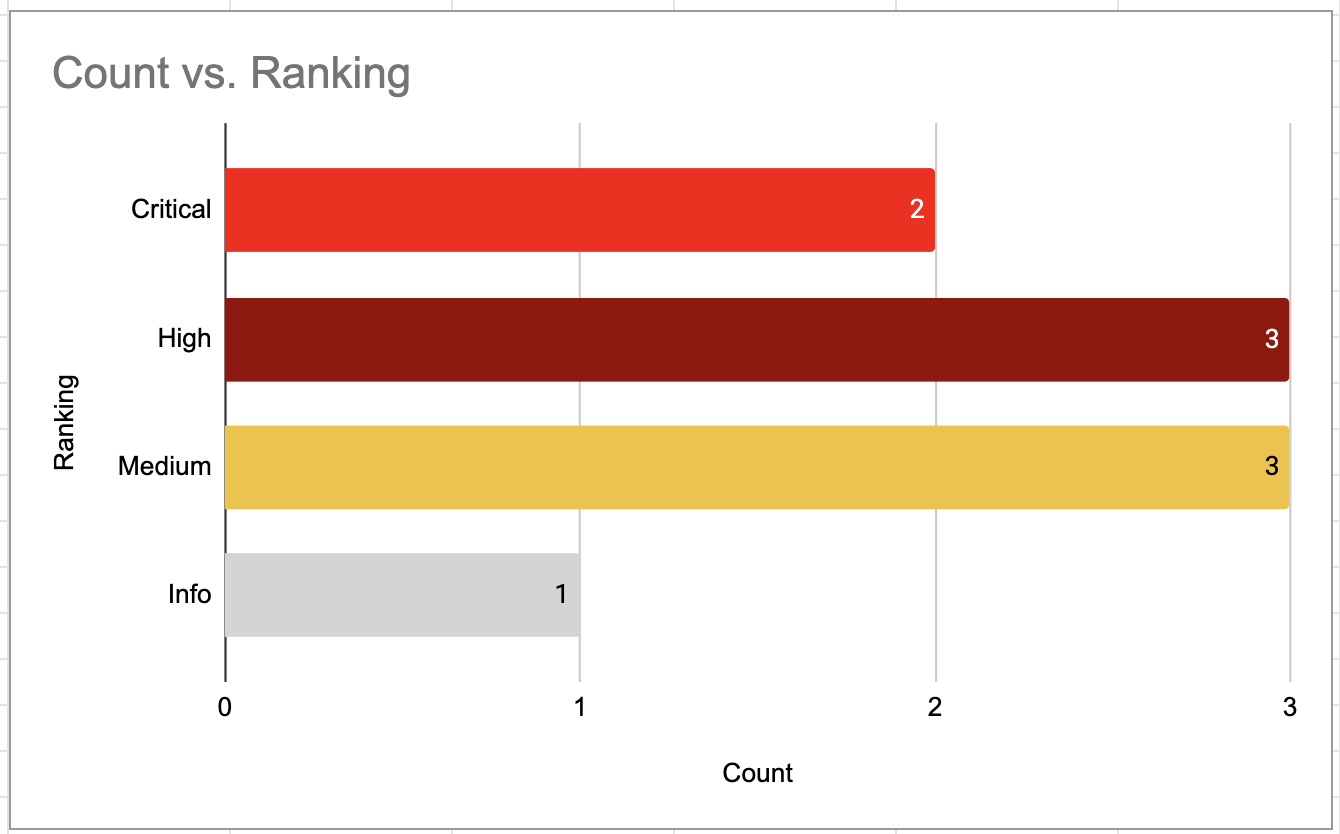
\includegraphics[width=\textwidth, height=350px]{pics/rankings.png}
\caption{Distribution of risks}\label{fig:bar_rankings}
\end{figure}


\newpage
\section{Key Findings}

List of security threats found in comparison to the baseline analysis are listed below:

\begin{enumerate}
    \item Phishing and social engineering of the mail servers.
    \item Denial of service due to some CVEs in the old database versions and mitigations like CDN also not present.
    \item Cross-Site Scripting as headers are not implemented in the CMS site.
    \item Security misconfigurations as many ports are made public unnecessarily.
    \item Ransomware attacks can be carried out with more ease, as important data-stores are open in public.
\end{enumerate}

\begin{figure}[htp!]
\centering
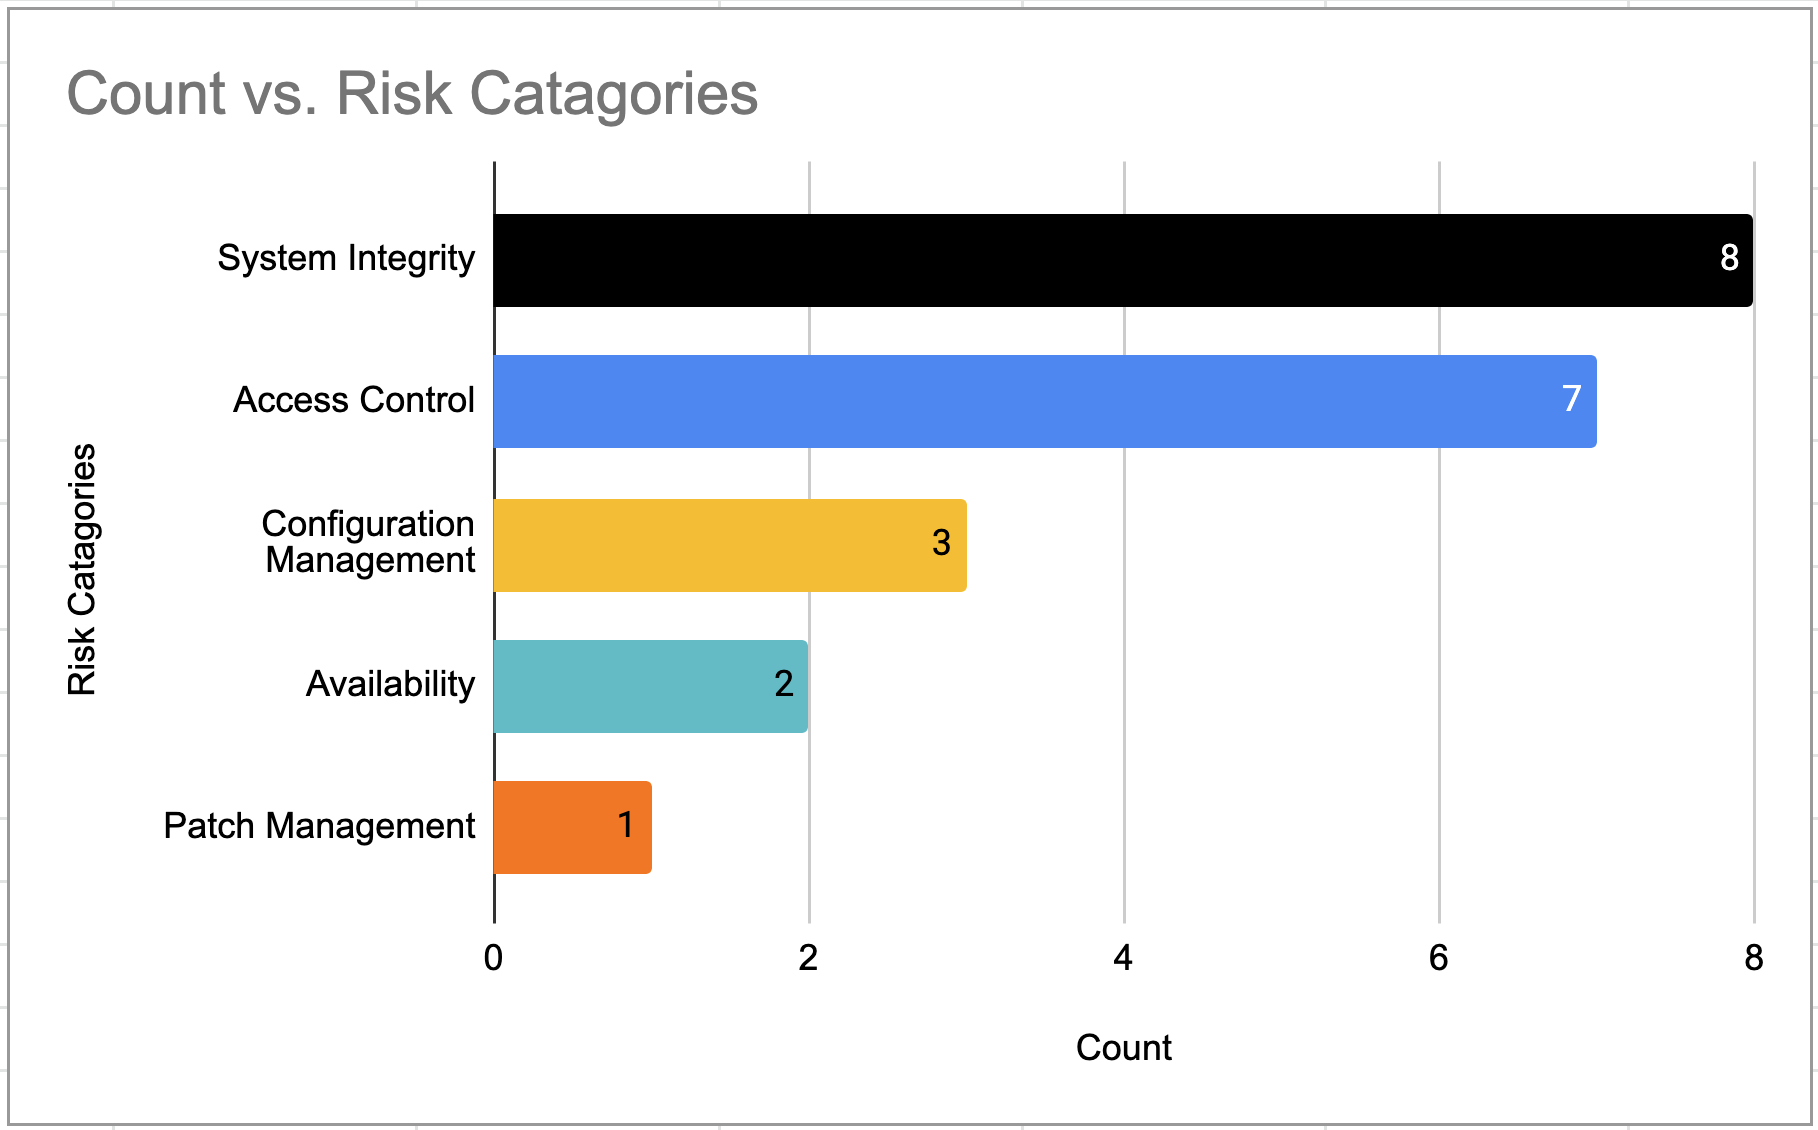
\includegraphics[width=\textwidth, height=330px]{pics/risk_cat.png}
\caption{Risk Catagories Count}\label{fig:bar_risks}
\end{figure}

\newpage
\begingroup
\centering
\setlength{\tabcolsep}{6.5pt} % Default value: 6pt
\renewcommand{\arraystretch}{1.8} % Default value: 1
\begin{longtable}{ |p{1.5cm}| p{6cm}|p{6.3cm}|}
\caption{Key Findings ordered by Priority}
    \label{table:key_findings}
\hline
\rowcolor{grey!15}
\textbf{Risk}  & \textbf{Finding}& \textbf{Recommendation}\\
\hline
\cellcolor{red!95} Critical  & Externally exposed Network Resources, i.e., databases, FTP, DNS servers. Information theft and DoS attacks can be performed with less effort.
 & Ports 21, 3306, and 5432 should be closed from the public internet as they are not necessary to be open for running the CMS. %CDN should be used to relieve the load on the servers.
\\
\hline
\cellcolor{red!95} Critical  & Privacy policy and cookie confirmation for users not available, therefore breaking GDPR directive. & A detailed cookie consent form and privacy policy, that a user can explicitly confirm to use the site should be implemented \citep[p.~2]{godr_cookie}.
\\
\hline
\cellcolor{red!55} High  & Insecure database versions  containing multiple CVEs. This can lead to personal data theft.
 & The vulnerable versions of the database must be updated to a secure one. In addition, regular security automatic scans with dynamic and static application testing should be carried out.
\\
\hline
\cellcolor{red!55} High  & Mail servers are unencrypted and could be intercepted, leading to a leak of sensitive information. & The mail servers should use TLSv1.3 to encrypt the traffic from getting intercepted during transit.\citep[p.~10]{tls_smtp}. 
\\
\hline
\cellcolor{red!55} High  & Malicious Code injection possible(XSS, CSRF forgery) & The HTML inputs should be sanitized, set Content-security policy header, and CSRF tokens \citep[p.~75]{xss_crsf}.
\\
\hline
\cellcolor{yellow!95} Medium  & Ip spoofing, DNS server spoofing, and Cache Poisoning possible.
& Implement DNSSEC to protect the integrity of the server and turn off DNS recursion in the Bind server. \citep[p.~38]{guo2006spoof}
\\
\hline
\cellcolor{yellow!95} Medium  & Server and application version is public.& Do not make server and application versions public information.
\\
\hline
\cellcolor{yellow!95} Medium  & DNS server is outdated and can cause an outage of the service because of present vulnerabilities..& Update DNS bind to v9.18.12.
\\
\hline
\cellcolor{grey!55} Info  & Mail server is not protected against spam and phishing.& A DMARC record in the DNS for the mail server should be included, which can validate the emails are from a genuine sender \citep[p.~7]{dmarc}.
\\
\hline
\end{longtable}
\endgroup

\newpage
\section{Conclusion}
Looking at table \ref{table:key_findings}, it can be concluded that the CMS system has severe critical flaws such as non-GDPR compliance because of missing privacy policies and consent, databases that might contain sensitive personal data are with open ports in the public internet. These errors pose a significant danger to the security operations of the system from attackers. Additionally, since the system is not GDPR conform, therefore is liable to be fined for not imposing the required elements. Herefore, the website is not production ready without resolving the high and critical issues from the findings.